\documentclass{article}
\usepackage{float}
\usepackage{graphicx}
\usepackage{flafter}

\begin{document}
\title{\vspace{-3.5cm}Least Asymmetry Algorithm}
\author{Dr. Nate Lust}
\maketitle
Least asymmetry was originally devised by James Gunn (Princeton
University) for use in radio astronomy. A non-exhaustive search through the
literature did not produce references, so we present the full
algorithm here.

We begin with an asymmetric distribution that is a result of the
optical aberrations in the system as well as the presence of noise in
the measured signal. Figure \ref{fig:pre_transform} depicts such an
asymmetric signal. We propose that the center is the point about which
the distribution is most symmetric. We define the asymmetry of the
signal as a function of position as

\begin{equation}
  \label{eq:asym}
  A(x,y) = \sum\limits_0^{R}Var(\Phi(r))*N(r),
\end{equation}
\noindent
where the discrete index $r$ indicates the particular radial bin, Var
is the variance operator, $\Phi$ is the flux, and $N(r)$ gives the
number of pixels at a given radius for weighting.  Equation
\ref{eq:asym} remaps images to a space in which the intensity is more
normally and symmetrically distributed, as demonstrated by fitting a
Gaussian to the image in asymmetry space {\em vs} flux space. In
principle, if this were a continuous dataset, we could continue this
process until the point of minimum asymmetry was absolutely
determined. Because datasets collected using imaging arrays are
discretely sampled, we take advantage of the increased symmetry and
use established centering routines to determine the point of minimum
asymmetry to sub-pixel accuracy.

To determine the point of minimum asymmetry, we calculate the
value of asymmetry about each pixel in the shaded region in Figure
\ref{fig:pre_transform}. The calculation begins by laying an aperture
about a given pixel as indicated in Figure
\ref{fig:pre_transform_with_ap}. This region, which we note extends
outside the window undergoing transformation, is used to create a
radial profile, (see Figure \ref{fig:profs}), with discrete radii
corresponding to the pixel centers, as shown in Figure
\ref{fig:circles}. The radial profile for the particular pixel shown
in Figure \ref{fig:pre_transform_with_ap} is given in Figure
\ref{fig:circlerad}. Because we only choose radii corresponding to
pixel centers, the radial bins are groupings of points at discrete
distances. As a general example of asymmetry, Figure \ref{fig:profs}
shows profiles corresponding to low (top) and high (bottom) asymmetry.

The generated radial profile is used in conjunction with Equation
\ref{eq:asym}, to calculate the value of asymmetry.  We repeat this
process for each pixel in the conversion window to produce the
asymmetry values depicted in Figure \ref{fig:asym_space}. Finally, we
use a traditional centering method in asymmetry space to determine the
center with sub-pixel accuracy. In our cursory tests, we determined
Gaussian centering performed better than center of light.

It is improper to do photometry on Figure \ref{fig:asym_space} as the
values correspond to sums of variances and not flux values. The figure
does not represent a cleaned up image but is merely an array
representation of the distribution of asymmetry values of the original
image. The center as determined from this distribution must be used in
flux space to determine photometric measurements.

\begin{figure}
  \centering
  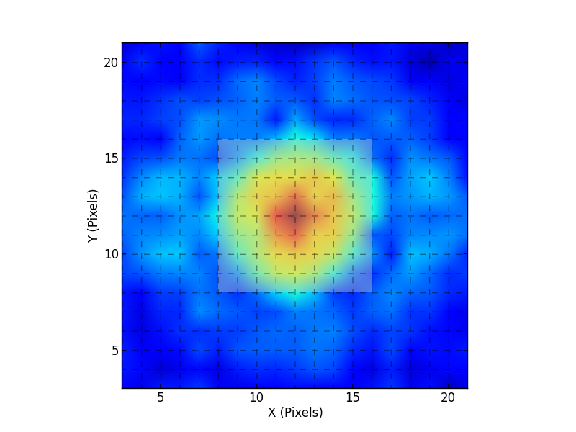
\includegraphics[width=0.5\textwidth]{f1.png}
  \caption{Asymmetric image for which the center is to be determined. The
    asymmetry value will be calculated for each pixel in the shaded
    region near the center of the image.}
  \label{fig:pre_transform}
\end{figure}

\begin{figure}
  \centering
  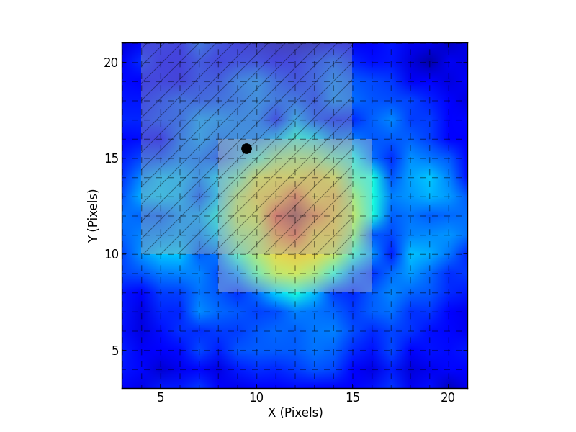
\includegraphics[width=0.5\textwidth]{f2.png}
  \caption{Asymmetric image with thatched region to indicate the region of
  transform for the dotted pixel}
  \label{fig:pre_transform_with_ap}
\end{figure}

\begin{figure}
\centering
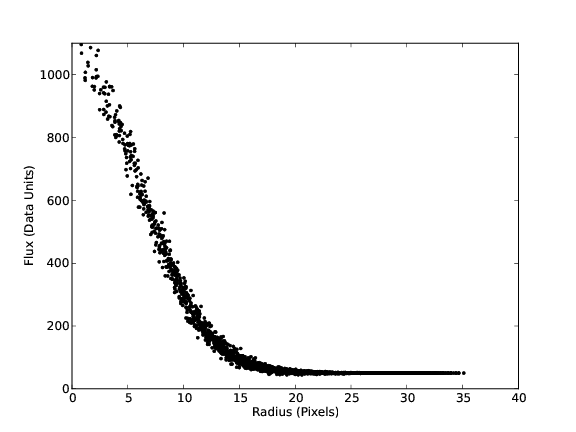
\includegraphics[width=0.38\textwidth]{f3a.png}\\
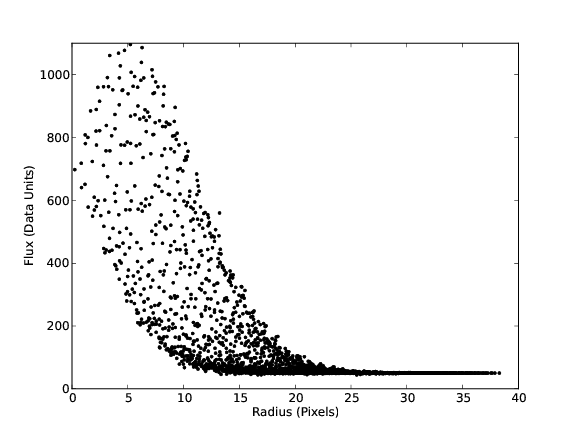
\includegraphics[width=0.38\textwidth]{f3b.png}
\caption{Stellar radial profiles. Top: When the profile is centered on
  the star, the variance in each radial bin is small, indicating low
  asymmetry. Bottom: When the profile is centered five pixels from
  the stellar center, the variance in each bin is high because the
  light is asymmetrically distributed about this point. The least
  asymmetry method works by minimizing the sum of the variances in all of
  the radial bins.}
\label{fig:profs}
\end{figure}

\begin{figure}
\centering
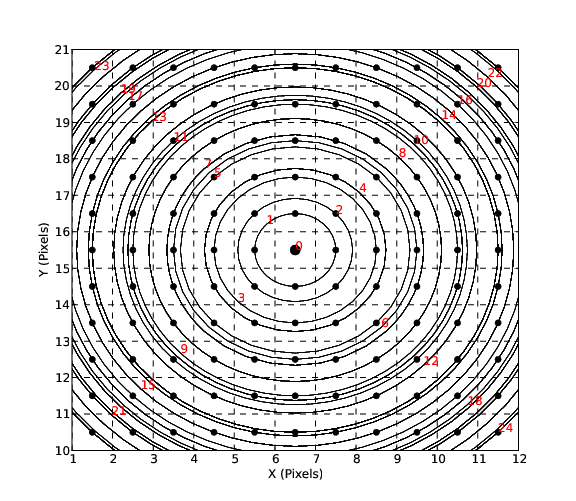
\includegraphics[width=0.5\textwidth]{f4.png}
\caption{Radii used to generate radial profile in the region of
  transformation.}
\label{fig:circles}
\end{figure}

\begin{figure}
\centering
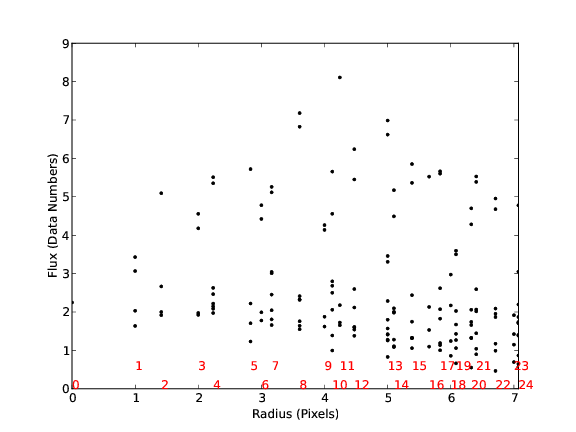
\includegraphics[width=0.5\textwidth]{f5.png}
\caption{Radial profile corresponding to our region of
  transformation. Red numbers correspond to the labels of radii shown
  in Figure \ref{fig:circles}}
\label{fig:circlerad}
\end{figure}

\begin{figure}
  \centering
  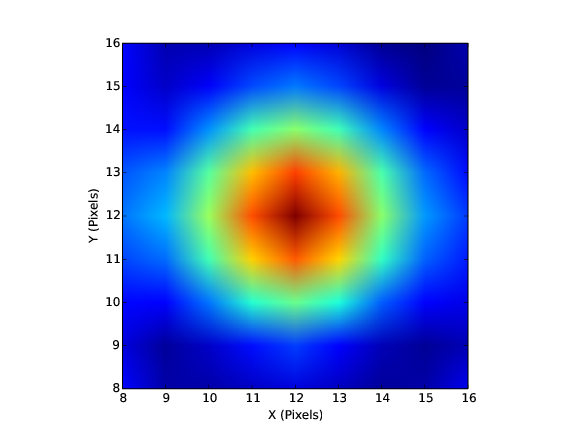
\includegraphics[width=0.5\textwidth]{f6.png}
  \caption{Image of asymmetry space for the region converted from
    Figure \ref{fig:pre_transform}.}
  \label{fig:asym_space}
\end{figure}
\end{document}
